\documentclass[12pt, xcolor=dvipsnames,svgnames,x11names]{article}
\usepackage{xcolor}
%\usepackage{universityos}
\usepackage{xspace}
\usepackage{url}
\usepackage[colorlinks=true,bookmarks=false,linkcolor=black,urlcolor=blue,citecolor=black]{hyperref}
\usepackage{fancyhdr}
\usepackage[top=1in,bottom=1in,left=1in,right=1in]{geometry}
\usepackage{multicol}
\usepackage{pgfplots}
\usetikzlibrary{circuits.logic.US}
% \usepackage{tgschola}
\let\temp\rmdefault
\usepackage{mathpazo}
\let\rmdefault\temp

\definecolor{roseRed}{HTML}{e20047}
\definecolor{coolGray}{HTML}{474747} % Neutral gray to contrast roseRed
\definecolor{mocha}{HTML}{a47864}
\definecolor{sage}{HTML}{8a9a5b}
\definecolor{dustyblue}{HTML}{6e8ca0}
\definecolor{terracotta}{HTML}{c87f5b}
\definecolor{lavender}{HTML}{9d8bb0}
\definecolor{darkmocha}{HTML}{7a5a4b}
\definecolor{darksage}{HTML}{667244}
\definecolor{darkdustyblue}{HTML}{526878}
\definecolor{darkterracotta}{HTML}{9e6347}
\definecolor{darklavender}{HTML}{766688}
\definecolor{winery}{HTML}{7e212a}

\definecolor{lightmocha}{HTML}{c2a190}
\definecolor{lightmocha1}{HTML}{d1b09c}
\definecolor{lightmocha2}{HTML}{e2c4b0}
\definecolor{lightmocha3}{HTML}{f0d9c7}

\definecolor{androidBlue}{HTML}{8AB4F8}
\definecolor{androidBlueLight}{HTML}{E8F0FE}
\definecolor{androidGreen}{HTML}{81C995}
\definecolor{androidGreenLight}{HTML}{E6F4EA}

% Red variants - based on Android's "error" and warning colors
\definecolor{androidRed}{HTML}{F28B82}
\definecolor{androidRedLight}{HTML}{FADAD7}

% Yellow variants - based on Android's accent/warning colors
\definecolor{androidYellow}{HTML}{FDD663}
\definecolor{androidYellowLight}{HTML}{FEF7E0}

% Purple variants - based on Android's system UI accents
\definecolor{androidPurple}{HTML}{D7AEFB}
\definecolor{androidPurpleLight}{HTML}{F4EAFC}

% Orange variants - based on Android's notification colors
\definecolor{androidOrange}{HTML}{FCAD70}
\definecolor{androidOrangeLight}{HTML}{FEEADC}

% Teal variants - based on Android's Material You palette
\definecolor{androidTeal}{HTML}{78D9EC}
\definecolor{androidTealLight}{HTML}{E6F6F9}

% Gray variants - based on Android's neutral colors
\definecolor{androidGray}{HTML}{DADCE0}
\definecolor{androidGrayLight}{HTML}{F1F3F4}

\usepackage{biolinum} % included with the {Libertine} font package
\renewcommand{\familydefault}{\sfdefault}



\usepackage[many]{tcolorbox}
\usepackage{CJKutf8}

\newcommand{\hw}{Classwork 02: Mathematical Preliminaries}
\newcommand{\duedate}{August 26, 2026}


% Redefine \maketitle to include tcolorbox
\makeatletter
\renewcommand{\maketitle}{%
    \begin{center}
        \begin{tcolorbox}[
            enhanced,
            colback=white,
            colframe=red!70!black,
            arc=0mm,
            title={\textcolor{white}{\bfseries CPE 381 \@title}},
            coltitle=white,
            fonttitle=\bfseries\large,
            attach boxed title to top left={xshift=10pt, yshift=-\tcboxedtitleheight/2},
            boxed title style={
            sharp corners,
            colback=red!70!black,
            frame hidden,
            boxrule=0pt,
            left=10pt, right=10pt,
            top=3pt, bottom=3pt
            }
        ]
        \large
        \vspace{10pt}
        \noindent Student Name (as in Canvas): \underline{\hspace{8cm}} 
        
        \vspace{10pt}
        \noindent A Number: \underline{\hspace{12cm}}

        \vspace{10pt}
        \noindent Points: 20 \quad Duration: 15 minutes \hfill \quad Due:~\duedate  ~(In-Class)

            \end{tcolorbox}
    \end{center}
}
\makeatother

\setlength{\parindent}{0pt}
\setlength{\parskip}{4pt}%

\input{common}


% Add showanswer toggle (set to "yes" for solutions, anything else for student version)
\usepackage{ifthen}
\newcommand{\showanswer}{yes}

\newenvironment{multiequation}[1][]{%
    \begin{equation}%
    \begin{aligned}%
        \ifx#1\@empty\else\label{#1}\fi%
}{%
    \end{aligned}%
\end{equation}% 
}
\pagestyle{fancy}

\lhead{\footnotesize{\coursenumber, \courseterm}, \footnotesize{The University of Alabama in Huntsville}}
\chead{}
\rhead{\footnotesize{\emph{\hw}}}
\lfoot{\footnotesize{Instructor: \instructorname}}
\cfoot{\footnotesize{\thepage}}
\rfoot{\footnotesize{\textit{Last Revised:~\today}}}
\renewcommand{\headrulewidth}{0.1pt}
\renewcommand{\footrulewidth}{0.1pt}
\newcommand{\minipagewidth}{0.8\columnwidth}

\renewcommand{\thefootnote}{\fnsymbol{footnote}}


\renewcommand{\headrulewidth}{0.1pt}
\renewcommand{\footrulewidth}{0.1pt}

\renewcommand{\thefootnote}{\fnsymbol{footnote}}

\usepackage{mdframed} 


\begin{document}


\title{\textsc{\hw}}

\author{Instructor: \instructorname}
\date{Due: \duedate}

\maketitle


\begin{enumerate}

\item Consider the complex number $z$ on Figure~\ref{fig:complex}. 
What is the complex conjugate $\overline{z}$? \hfill \textbf{(3 Points)}

\begin{figure}[htpb]
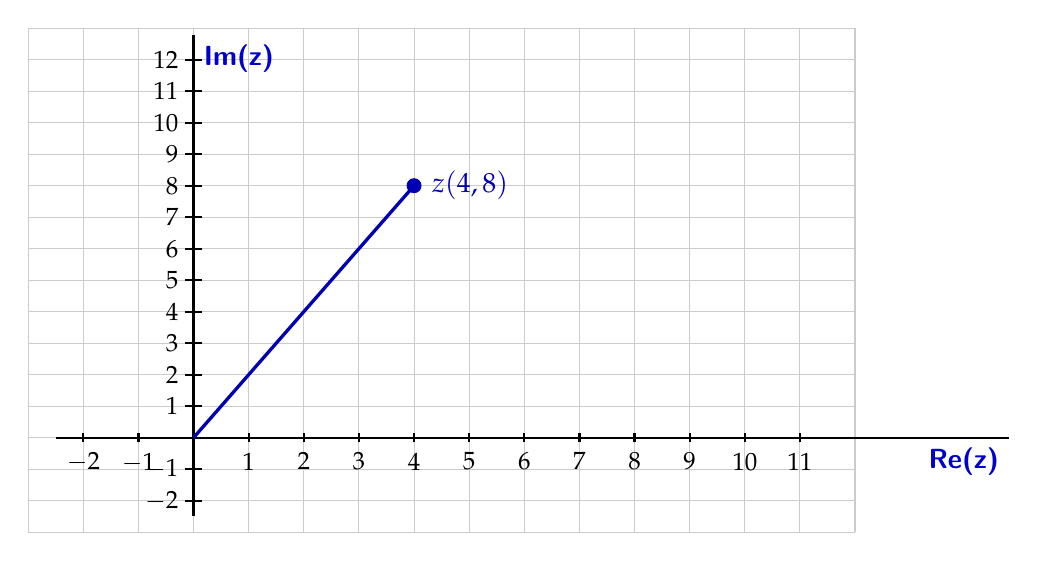
\begin{tikzpicture}[x=0.7cm, y=0.4cm]

    % Setting step=1 scales grid spacing to 1 unit (0.75cm) matching the tick marks
    \draw[gray!40, thin, step=1] (-3, -3) grid (12, 13);

    % Axes
    \draw[thick] (-2.5, 0) -- (14.8, 0) node[below left, color=blue!80!black, font=\bfseries] {Re(z)};
    \draw[thick] (0, -2.5) -- (0, 12.8) node[below right, color=blue!80!black, font=\bfseries] {Im(z)};

    % Horizontal Axis Ticks & Labels
    \foreach \x in {-2, -1, 1, 2, 3, 4, 5, 6, 7, 8, 9, 10, 11} {
        \draw[thick] (\x, -0.15) -- (\x, 0.15);
        \node[below=2pt, font=\small] at (\x, 0) {$\x$};
    }

    % Vertical Axis Ticks & Labels
    \foreach \y in {-2, -1, 1, 2, 3, 4, 5, 6, 7, 8, 9, 10, 11, 12} {
        \draw[thick] (-0.15, \y) -- (0.15, \y);
        \node[left=2pt, font=\small] at (0, \y) {$\y$};
    }

    % Vector from origin to z(4,8)
    \draw[line width=1.2pt, blue!70!black] (0, 0) -- (4, 8);

    % Target Point z(6,8)
    \filldraw[blue!70!black] (4, 8) circle (2.5pt);
    \node[right=3pt, color=blue!70!black, font=\bfseries] at (4, 8) {$z(4,8)$};

\end{tikzpicture}
\label{fig:complex}
\caption{Complex $z$.}
\end{figure}

\begin{tcolorbox}[
    enhanced,
    colback=androidBlueLight!80,
    colframe=androidBlue,
    arc=5pt,
    boxrule=1pt,
    title=\textbf{Answer},
    fonttitle=\bfseries,
    coltitle=black,
    top=10pt,
    bottom=8pt,
    left=8pt,
    right=8pt,
    attach boxed title to top left={xshift=10pt, yshift=-\tcboxedtitleheight/2},
    boxed title style={
    colback=androidBlue,    
        colframe=androidBlue,
        arc=3pt,
        boxrule=0pt,
        left=6pt, right=6pt,
        top=3pt, bottom=3pt
    }
    ]
    
    \vspace{1.0cm}
    ~
    
\end{tcolorbox}

\item If $z = \sqrt{3} + i$, what is $z^4$ in polar form? Use De Moivre’s Theorem. \hfill \textbf{(6 Points)}

\begin{tcolorbox}[
    enhanced,
    colback=androidBlueLight!80,
    colframe=androidBlue,
    arc=5pt,
    boxrule=1pt,
    title=\textbf{Answer},
    fonttitle=\bfseries,
    coltitle=black,
    top=10pt,
    bottom=8pt,
    left=8pt,
    right=8pt,
    attach boxed title to top left={xshift=10pt, yshift=-\tcboxedtitleheight/2},
    boxed title style={
    colback=androidBlue,    
        colframe=androidBlue,
        arc=3pt,
        boxrule=0pt,
        left=6pt, right=6pt,
        top=3pt, bottom=3pt
    }
    ]
    
    \vspace{5.0cm}
    ~
    
\end{tcolorbox}

\item What is the numerical value of $2(\sin^2 \theta + \cos^2 \theta)$? \hfill \textbf{(3 Points)}

\begin{tcolorbox}[
    enhanced,
    colback=androidBlueLight!80,
    colframe=androidBlue,
    arc=5pt,
    boxrule=1pt,
    title=\textbf{Answer},
    fonttitle=\bfseries,
    coltitle=black,
    top=10pt,
    bottom=8pt,
    left=8pt,
    right=8pt,
    attach boxed title to top left={xshift=10pt, yshift=-\tcboxedtitleheight/2},
    boxed title style={
    colback=androidBlue,    
        colframe=androidBlue,
        arc=3pt,
        boxrule=0pt,
        left=6pt, right=6pt,
        top=3pt, bottom=3pt
    }
    ]
    
    \vspace{1.0cm}
    ~
    
\end{tcolorbox}


\item If $\sin(\theta) = \frac{12}{13}$, and $\theta$ lies in the second quadrant, find the value of $\sec(\theta) + \tan (\theta)$. \hfill \textbf{(8 Points)}

\begin{tcolorbox}[
    enhanced,
    colback=androidBlueLight!80,
    colframe=androidBlue,
    arc=5pt,
    boxrule=1pt,
    title=\textbf{Answer},
    fonttitle=\bfseries,
    coltitle=black,
    top=10pt,
    bottom=8pt,
    left=8pt,
    right=8pt,
    attach boxed title to top left={xshift=10pt, yshift=-\tcboxedtitleheight/2},
    boxed title style={
    colback=androidBlue,    
        colframe=androidBlue,
        arc=3pt,
        boxrule=0pt,
        left=6pt, right=6pt,
        top=3pt, bottom=3pt
    }
    ]
    
    \vspace{15.0cm}
    ~
    
\end{tcolorbox}



\end{enumerate}


\end{document}